\chapter{Detección de obstáculos} \label{cap:detección_de_obstáculos}
% BREVE DESCRIPCIÓN DEL CONTENIDO DE ESTE CAPÍTULO
Este capítulo busca añadir mayor detalle a la caracterización del ambiente, en específico detectar objetos potencialmente peligrosos para el vehículo autónomo. Primero, en la sección \ref{sec:introducción_a_la_detección_de_ obstáculos}, se exponen aspectos básicos acerca de como un conductor puede detectar objetos en el camino. La sección, \ref{sec:algoritmos_de_agrupamiento} es una descripción de las categorías y características de los algoritmos de agrupación, mientras que la subsección, \ref{sub:ejemplo_para_obtener_una nube_de_puntos_con_ROS} es un ejemplo de como procesar una nube de puntos con ROS. Enseguida, la sección \ref{sec:el_algoritmo_K-medias} y subsección \ref{sub:ejemplo_de_implementación_del_algoritmo_K-medias} se enfocan en la definición teórica e implementación en código del algoritmo \textit{k-means} respectivamente. A continuación, la sección \ref{sec:empatado} habla acerca de la importancia de implementar un algoritmo de empatado. Finalmente, en \ref{sec:el_filtro_de_Kalman} se expone teóricamente el concepto de filtro de Kalman y \ref{sub:el_filtro_de_Kalman_extendido} su versión extendida, además, la subsección \ref{sub:estimación_de_posición_y_velocidad_con_el_filtro_de_kalman_extendido}, es un ejemplo de diseño e implementación de un filtro de Kalman para seguimiento de objetos.

Es importante mencionar que la implementación de códigos de este capítulo resulta en una combinación de lenguajes de programación C++ y Python, esta decisión se justifica y explica en las secciones correspondientes. Al finalizar este capítulo se muestran los resultados de las implementaciones aquí desarrolladas y en adición con la labor del seguimiento de carriles previamente diseñada, el vehículo autónomo no tripulado contará con un sistema más robusto que le permitirá tener una mejor percepción del ambiente.

\section{Introducción a la detección de obstáculos} \label{sec:introducción_a_la_detección_de_ obstáculos}

Los humanos pueden evitar obstáculos en el ambiente vehicular mientras manejan haciendo uso de los sentidos de la vista y oído. Con ellos, pueden percibir el ambiente y conocer si algún vehículo u obstáculo se encuentra al frente, por detrás o en los laterales. Es decir, conocen aunque con poca exactitud la posición de los obstáculos. Además, mediante la posición determinan que tan rápido avanzar para no chocar al frente, cuando comenzar a frenar en caso necesario e incluso fijar el ángulo de dirección en un rango estable para no chocar a los costados. Sin embargo, un vehículo autónomo no cuenta con un sistema que le permita realizar estas tareas de manera natural pues solo está instrumentado con sensores que le permiten conocer el ambiente. Con ayuda de algoritmos e instrumentos matemáticos y en combinación con información de sensores es posible simular estos comportamientos innatos para el ser humano.

El objetivo de este capítulo es contar con instrumentos que permitan determinar una situación donde intervenga la evasión de obstáculos a partir de dos tareas principales. En la sección anterior se mencionó la nula presencia de vehículos dentro del circuito de pruebas, ya es bien sabido que un ambiente vial cotidiano existen diversos objetos que podrían provocar colisiones. En específico, se buscan evitar accidentes del vehículo autónomo con otros vehículos dentro del circuito. Antes de definir una situación de evasión de objetos se requieren dos fases:
\begin{itemize}
    \item Detección de objetos
    \item Seguimiento de objetos
\end{itemize}
El objetivo de la detección es encontrar aquellos objetos potencialmente peligrosos para provocar cualquier tipo de accidente con el vehículo no tripulado, un escenario sencillo para navegación autónoma es usar las líneas del carril como guía dentro de un circuito cerrado. Sin embargo, en la búsqueda de situaciones más reales es importante considerar vehículos u otro tipo de objetos con diferentes tamaños, colores y obviamente posiciones distintas. La detección de objetos debe clasificar aquellos objetos que se encuentren dentro de la carretera pero en especial que impliquen un problema en la navegación del vehículo autónomo.

Una herramienta tecnológica en robótica que ayuda a ubicar objetos son los sensores láser. Como se mencionó en la subsección \ref{sub:sensores} un sensor LIDAR otorga puntos pertenecientes a una superficie. Este conjunto de puntos también conocido como nube de puntos no provee la información necesaria para decidir que objetos resultan un riesgo para el vehículo, por esta razón es necesario agrupar la nube de puntos en conjuntos que describan un objeto potencialmente peligroso y posteriormente determinar su posición. Las técnicas de agrupación tienen la capacidad de cumplir esta labor además, pueden trabajar con conjuntos grandes en tamaño para agruparlos en pequeños grupos de acuerdo a sus características. Dentro de la gran variedad de algoritmos de agrupación se encuentra el algoritmo \textit{k-means} que se caracteriza por agrupar bancos de datos en base a la cercanía (distancia) que existe entre ellos. 

Por otro lado, se entiende que los vehículos pueden desplazarse principalmente de manera vertical y en menor medida horizontalmente o por alguna razón pueden permanecer estáticos. Es evidente que los vehículos estáticos tienen velocidad $v = 0$,  mientras que la posición puede ser cualquier punto en el espacio pero constante. Sin embargo, en el caso contrario cuando la velocidad $v \neq 0$, la posición es distinta en cada momento y es proporcional a la velocidad que presente el vehículo. Este comportamiento implica la necesidad de predecir de alguna manera la velocidad y posición de vehículos estáticos y en movimiento. El seguimiento de vehículos tiene el objetivo de cumplir esta meta con ayuda de un instrumento matemático conocido como filtro de Kalman, el cual permite predecir estados futuros de un sistema dinámico.

Cada una de estas fases tienen desarrollos distintos, los cuales son:
\begin{itemize}
    \item Detección de objetos
        \begin{enumerate}
            \item Obtener la nube de puntos otorgada por el sensor LIDAR.
            \item Agrupar la nube de puntos.
            \item Obtener la posición de cada objeto detectado.
        \end{enumerate}
    \item Seguimiento de objetos
    \begin{enumerate}
        \item Diseñar un sistema dinámico que involucre posición y velocidad.
        \item Estimar posiciones y velocidades futuras de cada objeto.
    \end{enumerate}
\end{itemize}

La combinación de detectar y seguir obstáculos es esencial para iniciar con la tarea específica de evasión de obstáculos. 

\section{Algoritmos de agrupamiento} \label{sec:algoritmos_de_agrupamiento}

Existe una gran variedad de algoritmos de agrupación y por ello, resulta complicado hacer una clasificación exacta de estos métodos porque algunas categorías podrían superponerse con otras, de modo que, un algoritmo puede poseer características de una o varías categorías. No obstante, es de mucha utilidad crear una organización relativa para los métodos de agrupamiento existentes. Los principales algoritmos de agrupación pueden ser clasificados en las siguientes categorías \cite{han2011data}.

\begin{enumerate}
    \item \textbf{Métodos de división:} Centran su funcionamiento en el calculo de distancias por ejemplo, distancia de \textit{Manhattan} o distancia Euclidiana (\ref{eqn:euclidian_distance}). Dado un conjunto de $n$ objetos, un método de división construye $k$ divisiones. Cada división representa un \textit{cluster} o grupo con $k \leq n$. Este tipo de algoritmos agrupan los datos en $k$ \textit{clusters} y cada \textit{cluster} contiene al menos un objeto.
    
    Sea $k$ el número de divisiones a construir, el método de división crea una división inicial. Después usa una técnica de reubicación iterativa que busca mejorar el agrupamiento moviendo los objetos de un grupo a otro. El criterio general para asignar objetos en un grupo es que tan cerca o relacionados están los objetos de un grupo, mientras que objetos en diferentes \textit{clusters} se mantienen lejanos o son muy diferentes. \textit{k-means} y \textit{k-medoids} son ejemplos de esta técnica de agrupación. Estos métodos funcionan bien para agrupar conjuntos con formas esféricas en conglomerados de tamaño pequeño o mediano. Para formar grupos con formas complejas y con conjuntos de mayor tamaño, es necesario mejorar o buscar otros métodos.
    
    \item \textbf{ Métodos jerárquicos:} Un método jerárquico se caracteriza por crear una descomposición jerárquica del conjunto de datos inicial en objetos de datos. Los métodos jerárquicos se pueden clasificar según la estrategia que implementan, ya sea aglomerativa o divisiva. También conocido como enfoque de abajo hacia arriba, el método de aglomeración comienza formando un grupo por cada objeto para después fusionar los objetos o grupos cercanos entre sí, hasta que todos los grupos forman uno solo o bien se cumple una condición de paro. El enfoque divisivo, igualmente llamado enfoque de arriba hacia abajo, inicia con todos los objetos dentro de un grupo. Luego, un grupo se divide en grupos más pequeños por cada iteración hasta que cada objeto está en un grupo o una condición de paro se cumpla.
    
    Los métodos jerárquicos cuentan con una condición de rigidez porque una vez que un paso de combinación o división es realizado no se puede anular. Sin embargo, esta desventaja es aprovechada por provocar menores costos de cálculo al no tener preocupación por un número de diferentes combinaciones. Una desventaja más de estas técnicas radica en que no pueden corregir decisiones erróneas.
    
    \item \textbf{ Métodos basados en densidad:} Uno de las principales inconvenientes de los métodos de agrupación por división es que solo funcionan bien para encontrar formas esféricas mientras que estructuras arbitrarías resulta una tarea difícil. Otros métodos de agrupación han sido desarrollados bajo la noción de densidad (número de objetos o puntos de datos). Su idea general consiste en incrementar un determinado grupo siempre y cuando la densidad de una vecindad exceda un umbral. Es decir, para cada punto contenido en un grupo, la vecindad debe de contener un mínimo de puntos.
    
    Este tipo de métodos son útiles para reducir ruido en valores atípicos provocados por lecturas de sensores además de descubrir grupos con formas arbitrarias.
    
    \item \textbf{Métodos basados en cuadrículas:} Los métodos basados en cuadrículas se pueden integrar con distintos métodos de agrupación, como los métodos basados en densidad y los métodos jerárquicos, a menudo resulta eficiente el uso de cuadrículas en muchas aplicaciones de la minería de datos. El agrupamiento por cuadrículas cuantifica el espacio de un objeto en un número finito de celdas que forman una estructura de cuadrícula, todas las operaciones de agrupación son realizadas dentro de la cuadrícula, es decir, el espacio cuantificado. La principal ventaja de este método es el bajo coste computacional y rápido tiempo de procesamiento, pues por lo general es independiente del número de datos a agrupar y solo depende de la cantidad de celdas en cada dimensión dentro del espacio cuantificado.
\end{enumerate}

\begin{equation}
    d_E(P_1, P_2) = \sqrt{(x_1 - x_2)^2 - (y_1 - y_2)^2}
    \label{eqn:euclidian_distance}
\end{equation}

Algunos de los algoritmos de agrupación integran ideas de distintos métodos, por lo que en ocasiones es difícil colocar un algoritmo dentro de una categoría específica. Además, algunas aplicaciones llegan a presentar criterios que requieren de más de un método de agrupación. El cuadro \ref{tab:clustering_methods} muestra las principales características las clasificaciones antes descritas. En este trabajo se utilizará un método de agrupación por división, ver sección \ref{sec:el_algoritmo_K-medias}.
\begin{table}[t]
    \begin{center}
    \begin{tabular}{| l | l |}
    \hline
    Método & Características Principales \\ \hline
    De división & Basado en distancia \\ & Efectivo en conjuntos pequeños y medianos \\ & Utiliza la media o medoides para representar \\ & el centro de un \textit{cluster}  \\ \hline
    Jerárquico & Puede incorporar otras técnicas \\ & El agrupamiento es una descomposición \\ & jerárquica \\ & No corrige después de una combinación o \\ & división \\ \hline
    Basado en densidad  & Encuentran formas arbitrarias \\ & Filtran valores atípicos  \\ & Cada punto debe tener un mínimo de \\ & puntos dentro de su vecindad \\ \hline
    Basado en cuadrículas & Una cuadrícula es la estructura de datos \\ & Es más rápido que otros métodos \\ \hline
\end{tabular}
    \end{center}
    \caption{Clasificaciones de algoritmos de agrupamiento y sus principales características.}
    \label{tab:clustering_methods}
\end{table}

\subsection{Ejemplo para obtener una nube de puntos con \textit{ROS}} \label{sub:ejemplo_para_obtener_una nube_de_puntos_con_ROS}

El primer paso en la detección de objetos es contar con un instrumento que permita caracterizar el ambiente que rodea al vehículo de pruebas. Webots tiene la facilidad de simular diferentes sensores que instrumentan el vehículo de forma independiente, de manera similar a la cámara existe un nodo específico en el simulador para seleccionar un sensor LIDAR de un amplío catálogo que incluye algunas de las marcas y modelos más comerciales como: Velodyne, SICK, Hokuyo y Robotis. Sin embargo, Webots también ofrece la posibilidad de caracterizar un nodo LIDAR con las características únicas y necesarias para propósitos específicos. Está flexibilidad es una gran ventaja porque permite especificar los parámetros requeridos que mejor se ajusten a la aplicación en turno.

De este modo, los principales parámetros requeridos del sensor LIDAR a usar son:
\begin{itemize}
    \item \textbf{Campo de visión horizontal:} $2\pi = 360^{\circ}$
    \item \textbf{Resolución horizontal:} 1024 puntos por capa
    \item \textbf{Campo de visión vertical:} $0.3^{\circ}$, ángulo entre primera y última capa
    \item \textbf{Número de capas:} 16
    \item \textbf{Rango máximo:} 30[m]
\end{itemize}

Otra razón para usar un sensor LIDAR convencional y con parámetros específicos es qué se tiene un mayor control sobre el número de puntos otorgados por el sensor, pues esta característica es de vital importancia para el desempeño de un algoritmo de clusterización.

De manera similar a la imagen de la cámara descrito en el capítulo \ref{cap:seguimiento_de_carriles}, pero con las diferencias necesarias se pretende obtener la información del sensor LIDAR, en específico la nube de puntos. El proceso para obtener la nube de puntos del sensor requiere un mensaje tipo \textit{PointCloud2}, las parámetros más importantes de este mensaje incluyen: alto y ancho de la nube de puntos, tamaño de una fila y de cada punto en bytes además de la propia nube de puntos en cada momento, etc. Cada uno de los parámetros requeridos por el mensaje \textit{PointCloud2} contienen los valores recomendados en las documentaciones de Webots y \textit{ROS}, el parámetro más importante de este mensaje es \textit{data} y debe de contener una estructura del tipo \textit{bytearray} por recomendación de la propia documentación, ya que usar una lista convencional tiene la desventaja de ser más lento entre más puntos contenga la nube de puntos. El controlador principal del vehículo de pruebas desarrollado en Python propone el siguiente código para este efecto.

\hfill
\begin{lstlisting}[language=Python]
# INIT LIDAR
lidar = Lidar('lidar')          
lidar.enable(TIME_STEP)
lidar.enablePointCloud()

# POINT CLOUD2 MESSAGE 
msg_point_cloud = PointCloud2()
msg_point_cloud.header.stamp = rospy.Time.now()
msg_point_cloud.header.frame_id = 'lidar_link'  
msg_point_cloud.height = 1
msg_point_cloud.width = lidar.getNumberOfPoints()
msg_point_cloud.point_step = 20
msg_point_cloud.row_step = 20 * lidar.getNumberOfPoints()
msg_point_cloud.is_dense = False
msg_point_cloud.fields = [
    PointField(name = 'x', offset = 0, datatype = PointField.FLOAT32, count = 1),
    PointField(name = 'y', offset = 4, datatype = PointField.FLOAT32, count = 1),
    PointField(name = 'z', offset = 8, datatype = PointField.FLOAT32, count = 1),
]
msg_point_cloud.is_bigendian = False
msg_point_cloud.data = lidar.getPointCloud(data_type='buffer')       
\end{lstlisting}
\hfill

Con el mensaje \textit{PointCloud2} se define un tópico que publica el contenido del mensaje, posteriormente se debe agrupar la nube puntos con un algoritmo de agrupación, también se usa el mensaje para tener una visualización de la nube de puntos a través del visualizador RViz de \textit{ROS}. Este paquete tiene la particularidad de recibir múltiples mensajes de sensores disponibles en \textit{ROS} y realizar visualizaciones 3D de estos. 

La imagen \ref{fig:pc_webots} muestra la nube de puntos vista desde el simulador. A manera de respaldar el resultado del código anterior se presenta la misma nube de puntos pero en el visualizador RViz, ver \ref{fig:pc_rviz}.
\begin{figure}[h]
    \centering
    \begin{subfigure}[b]{0.4\textwidth}
         \centering
         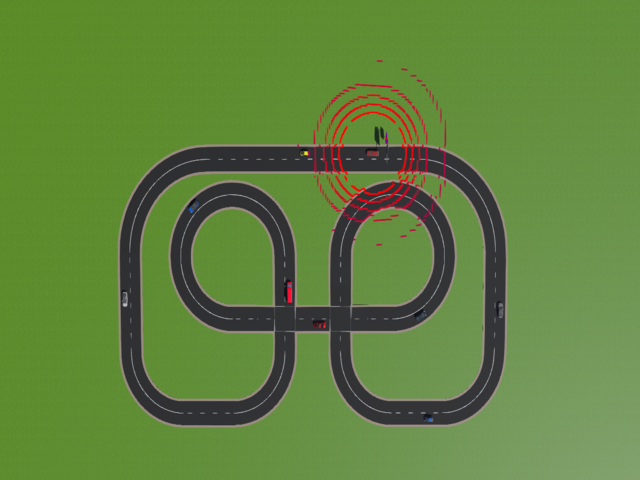
\includegraphics[width=\textwidth]{Figures/Figures_Cap05/pc_webots.png}
         \caption{Nube de puntos en Webots.}
         \label{fig:pc_webots}
    \end{subfigure}
    \hfill
    \begin{subfigure}[b]{0.4\textwidth}
         \centering
         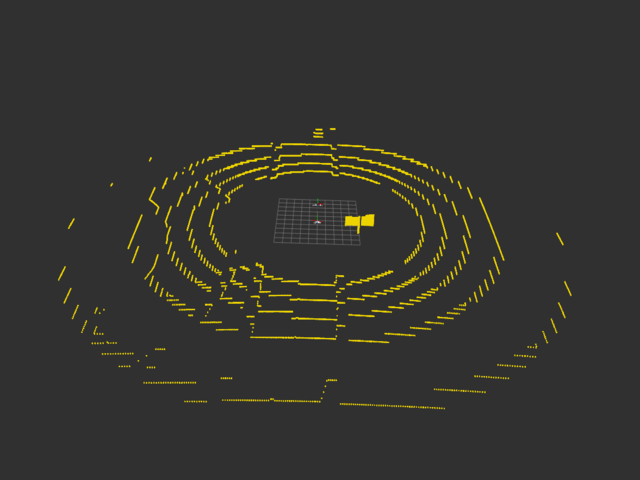
\includegraphics[width=\textwidth]{Figures/Figures_Cap05/pc_rviz.png}
         \caption{Nube de puntos en Rviz.}
         \label{fig:pc_rviz}
     \end{subfigure}
     
    \caption{Nube de puntos en Webots y Rviz.}
    \label{fig:pc_webots_rviz}
\end{figure}

\section{El algoritmo K-medias} \label{sec:el_algoritmo_K-medias}

La versión más simple y fundamental para el análisis de grupos es la división, organiza objetos de un conjunto en varios grupos o \textit{clusters}. Para mantener la especificación del problema, se entiende que el número de \textit{clusters} iniciales se proporciona con conocimiento previo ya que este parámetro es el punto de partida en cualquier método de agrupación por división.

Sea \textit{D} un conjunto de datos, con \textit{n} objetos, y \textit{k}, el número de grupos por formar, un algoritmo de agrupación por división ordena los objetos en \textit{k} particiones con $k \leq n$, donde cada partición representa un grupo. Los \textit{clusters} se forman a partir de una función de disimilitud basada en distancia como criterio, objetos contenidos en un \textit{cluster} son similares entre sí pero diferentes a los objetos de otros \textit{clusters}. Dado un conjunto \textit{D} con \textit{n} objetos en el espacio euclidiano. Los métodos de división distribuyen los \textit{n} datos de \textit{D} en \textit{k} grupos $C_1, C_2, C_3,..., C_k$. Se utiliza una función objetivo para evaluar la partición de la división. Es decir, la función objetivo busca una alta similitud dentro de un grupo y una baja similitud con grupos externos.

El algoritmo \textit{k-means} es una técnica de división basada en centroide, dicho de otra manera utiliza el centroide $c$ para representar un grupo $C$. Teóricamente, el centroide de un \textit{cluster} es su punto central. La definición de centroide puede ser de distintas maneras, como la media o medoide de los puntos u objetos asignados al grupo.

La diferencia entre un objeto $p_i \in C_i$ y su centroide $c_i$ se mide como $d(p_i, c_i)$, donde $d$ es la distancia euclidiana entre dos puntos en $[x, y]$. La calidad del \textit{cluster} $C_i$ se puede medir como la variación del grupo, que es la suma del error cuadrático entre todos los objetos $p_i$ en $C_i$ y el centroide $c_i$, como:
\begin{equation}
    E = \sum_{i=1}^{k}\sum_{p\in{C_i}}d(p_i, c_i)^2
\end{equation}

donde \textit{E} es la suma del error cuadrático de todos los puntos en el conjunto de datos, $p_i$ es un punto en el espacio que representa un objeto; y $c_i$ es el centroide del \textit{cluster} $C_i$. Dicho de otra manera, la distancia desde un punto hacia el centro de su grupo se eleva al cuadrado y las distancias se suman. El propósito de esta función objetivo es hacer que los \textit{k} \textit{clusters} resultantes sean lo más separados y compactos posibles, \textit{k-means} establece el centroide de un \textit{cluster} como el valor medio de los puntos que contiene. 

Al comenzar, \textit{k-means} selecciona aleatoriamente \textit{k} objetos de \textit{D}, cada uno de estos representa inicialmente un centro o media de \textit{cluster}. Todos y cada uno de los objetos $p_i$ restantes se reasignan al grupo que más sean similares en función de la distancia euclidiana que existe entre el punto $p_i$ y la media de grupo $c_i$. En otras palabras, cada objeto $p_i$ se une al grupo $C_i$ más cercano y $c_i$ representa la media de todos los objetos que contiene $C_i$. Después, el algoritmo mejora iterativamente la variación dentro del grupo calculando una nueva media de los objetos asignados al \textit{cluster} en la iteración anterior. En breve, todos los objetos se reasignan utilizando el valor medio de cada \textit{cluster} como el nuevo centroide $c_i$ de $C_i$. El proceso iterativo se repite hasta que la asignación es estable, es decir, los grupos formados en la ronda actual son los mismos que se formaron en la ronda anterior. Dicho de otro modo, la diferencia entre $c_i$ anterior y $c_i$ actual es mínima. El algoritmo \ref{alg:k-means} describe este proceso.
\begin{algorithm}
    \begin{algorithmic}[0]
        \REQUIRE $k:$ Número de \textit{clusters} \\ \parindent=12.5mm $D:$ Conjunto de datos con $n$ objetos
        \ENSURE $k$ centroides
        \STATE Obtener centroides iniciales $C = \{c_0, c_1, .... , c_k\}$ con $k$ objetos de $D$
        \FORALL{$p$ en $D$}
            \STATE Calcular $d(p_i, c_i) = \sqrt{(p_{i_{x}} - c_{i_{x}})^2 + (p_{i_{y}} - c_{i_{y}})^2 (p_{i_{z}} - c_{i_{z}})^2}$
            \STATE Añadir $p_i$ al \textit{cluster} $c_i$ más cercano
        \ENDFOR
        \STATE Obtener nuevos centroides $C_n = \{\bar{c_0}, \bar{c_1}, .... , \bar{c_k}\}$
        \STATE Calcular $\Sigma d(C, C_n)$.
        \WHILE{$\Sigma d(C, C_n) > tolerancia$}
            \STATE Actualizar $C$ $\leftarrow$ $C_n$
            \STATE Reagrupar $p_i$ en $c_i$
            \STATE Recalcular $C_n = \{\bar{c_0}, \bar{c_1}, .... , \bar{c_k}\}$
            \STATE Recalcular $\Sigma d(C, C_n)$
        \ENDWHILE
        \RETURN $k$ centroides
    \end{algorithmic} 
  
    \caption{Algoritmo \textit{K-means}.}
    \label{alg:k-means}
\end{algorithm}

Sin embargo, no se garantiza que \textit{k-means} converja a un óptimo global y en muchos de los casos termina en un óptimo local. Por otro lado, el resultado de la agrupación puede depender de la selección aleatoria inicial de centroides. En la práctica, para obtener mejores resultados es común ejecutar el algoritmo \textit{n} veces con diferentes centroides iniciales. La complejidad de \textit{k-means} es de $O(nkt)$; donde \textit{n} es total de objetos, \textit{k} es el número de \textit{clusters} a formar y \textit{t} el número de iteraciones. Por lo tanto, este método es relativamente escalable para grandes conjuntos de datos.

El método \textit{k-means} no resulta adecuado para descubrir formas arbitrarias. Además, es sensible al ruido y a datos atípicos pues pueden influir sustancialmente en el valor medio. Existen diferentes variantes del método \textit{k-means} que pueden diferir en la selección de los \textit{k} \textit{clusters} iniciales, el cálculo de la disimilitud y estrategias para calcular la media de los \textit{clusters}.

\subsection{Ejemplo de implementación del algoritmo K-medias} \label{sub:ejemplo_de_implementación_del_algoritmo_K-medias}

El segundo paso en la detección de objetos es implementar un algoritmo de agrupación, como se mencionó anteriormente el algoritmo \textit{k-means} es el elegido para agrupar la nube de puntos del sensor LIDAR y lograr la detección de objetos, en específico vehículos. Debido a que el sensor LIDAR está situado en la parte superior del vehículo, ver \ref{fig:webots_car}, es importante delimitar el área donde existan puntos de interés en la búsqueda de objetos potencialmente peligrosos. En breve se enuncia el proceso para agrupar la nube de puntos.   
\begin{enumerate}
    \item Eliminar puntos que pertenezcan al suelo del escenario.
    \item Definir el número de \textit{clusters} iniciales que serán los encargados de identificar obstáculos.
    \item Aplicar \textit{k-means} al conjunto de puntos previamente filtrado.
\end{enumerate}

En un primer intento por implementar el algoritmo \textit{k-means} se usó Python como lenguaje de programación donde se logró el objetivo de obtener los centroides que indican la posición de cada objeto contenido en la escena. Sin embargo, se presentaron algunos inconvenientes en los resultados finales, por ejemplo: 
\begin{itemize}
    \item La posición de los centroides no es constante con la posición de los objetos. Es decir, la posición de los centroides  varía en cada momento aún cuando los objetos permanecen estáticos.
    \item La velocidad del algoritmo incrementa conforme crece el tamaño de la nube de puntos.
\end{itemize}

Para lidiar con estos inconvenientes se decide hacer una nueva implementación del algoritmo \textit{k-means} pero ahora en lenguaje de programación C++ con el fin de tener más control en cada una de las operaciones que involucra el algoritmo además de disminuir el tiempo de procesamiento del mismo.

Para completar el primer requisito del agrupamiento es necesario filtrar la nube de puntos y eliminar puntos pertenecientes al suelo. Es difícil tener una medición exacta que permita delimitar la altura que existe desde el suelo hasta la posición del sensor LIDAR. Debido a esto mediante experimentación se llega al valor de $-1.5[m]$ en el eje $y$ que representa la altura en el sistema coordenado, este valor en $y$ es un umbral que delimita puntos que forman el suelo y puntos que no son parte de él. Es decir, todos los puntos $ y<-1.5$ son despreciados, además se eliminan puntos con valor $inf$ o $NaN$ de la nube de puntos para evitar posibles errores en operaciones posteriores del algoritmo \textit{k-means}. 

En breve se ejemplifica la implementación en código, donde las líneas 2 y 3 muestran las condiciones para eliminar puntos $inf$ y suprimir puntos perteneciente al suelo respectivamente.

\hfill
\begin{lstlisting}[language=C]
void objectDetectCallback(const sensor_msgs::PointCloud2::ConstPtr& msg){
    if( (isinf(x) or isinf(y) or isinf(z)) != true){
        if( y > -1.5 ){
            std::vector<double> point = {x, y, z};
            point_cloud.push_back(point);
        }
    }
}
\end{lstlisting}
\hfill

Definir el número de \textit{clusters} considerados para el algoritmo \textit{k-means} es una ardua tarea en esta aplicación, pues el propósito general es detectar autos y en un ambiente vial existen múltiples situaciones con un número diferente de vehículos en cada situación, como consecuencia de este hecho no se puede definir a priori la cantidad de grupos iniciales que mejor se ajuste a cada una de las situaciones, porque existen una infinidad de casos. Aunque el método del codo o \textit{elbow-method} del algoritmo \textit{k-means} es una herramienta de utilidad que funciona en otro tipo aplicaciones pero, para este caso en particular resulta costoso en tiempo de procesamiento debido a que la nube de puntos cambia mientras el vehículo se desplaza vertical u horizontalmente.

Sin embargo, uno de los propósitos de este trabajo es probar cada uno de los algoritmos bajo un ambiente supervisado y controlado, tal y como se hizo con el circuito de prueba para detección y seguimiento de carril donde el vehículo de pruebas está dentro de un circuito cerrado también se añade un número invariable de vehículos con el objetivo de realizar pruebas en la detección de objetos de manera controlada.  Siguiendo este enfoque se pretende añadir un máximo de 5 diferentes vehículos con distintas posiciones en el circuito de pruebas, por lo tanto el número mínimo de \textit{clusters} iniciales debe de ser $\geq 5$.
\newpage

Con los dos pasos realizados previamente se puede comenzar la implementación del algoritmo \textit{k-means} para agrupar la nube de puntos, como se mencionó anteriormente la implementación en código de este algoritmo es en lenguaje C++ por razones ya explicadas, la implementación corresponde directamente al algoritmo \ref{alg:k-means} y se tienen en cuenta las siguientes consideraciones.
\begin{enumerate}
    \item La agrupación de puntos se define a través de la cercanía que existe entre ellos.
    \item El número y posición de los \textit{clusters} iniciales es definido antes de iniciar el agrupamiento.
    \item La cercanía entre puntos es calculada con distancia euclidiana.
    \item Si un grupo no contiene puntos entonces es ignorado.
    \item Si dos centroides se encuentran a distancia mínima se obtiene el promedio de ambos que resulta en uno solo.
    \item La condición de paro del algoritmo es el cambio mínimo de posición de los centroides o cuando se exceda un máximo de intentos.
\end{enumerate}

\begin{lstlisting}[language=C]
/* KMEANS FUNCTION */
std::vector<std::vector<double>> kmeans(std::vector<std::vector<double>> point_cloud){

    new_centroids = calulate_centroids(point_cloud, initial_centroids);        
    total_distance = compare_centroids(new_centroids, initial_centroids);      

    while (total_distance > tol && attemps < max_attemps){
        std::vector<std::vector<double>> centroids(new_centroids); 
        new_centroids = calulate_centroids(point_cloud, centroids); 
        total_distance = compare_centroids(new_centroids, centroids);
        attemps += 1;
    }
    return new_centroids;                                            
}
\end{lstlisting}
\hfill

La función \textit{kmeans} del código anterior recibe como parámetro una nube puntos y el valor de retorno es el conjunto de centroides calculados, es decir, la posición media de cada uno de los grupos formados por el algoritmo.

Las líneas más importantes del código anterior son explicadas a continuación:
\begin{itemize}
    \item La línea 4 efectúa el agrupamiento para cada punto de la nube y calcula la media de cada centroide por medio de la función \textit{calculate\_centroids()}. Donde el primer parámetro es la nube de puntos y el segundo parámetro corresponde al conjunto de centroides iniciales previamente establecidos.
    \item La línea 5 realiza el calculo de distancia euclidiana total entre centroides actuales e iniciales.
    \item A partir de la línea 7 se inicia un ciclo para repetir el agrupamiento hasta que se cumpla una de las condiciones de paro.
    \item La línea 8 realiza una copia los nuevos centroides para efectuar el siguiente calculo con el valor actualizado. Mientras que 9 y 10 realizan agrupamiento y calculo de distancia entre centroides respectivamente.
\end{itemize}

Al finalizar este proceso se obtiene como resultado un conjunto de centroides que corresponden a la posición media de los grupos formados por el algoritmo de agrupación. La posición de cada centroide se expresa en coordenadas cartesianas en un espacio de tres dimensiones $(x, y, z)$. En conclusión, al finalizar el proceso de agrupación se adquieren las posiciones medias (centroides) de los objetos detectados en la nube de puntos. En \ref{fig:pc_centroids} se ilustra este resultado con el visualizador RViz, donde los puntos amarillos forman la nube de puntos y los centroides correspondientes a cada objeto en color rojo. Si se observa \ref{fig:pc_clustering} con detenimiento se puede verificar que las posiciones de los centroides se encuentran en un punto medio de cada objeto sin tomar en consideración puntos pertenecientes al piso del escenario.
\begin{figure}[h]
    \centering
    \begin{subfigure}[b]{0.45\textwidth}
         \centering
         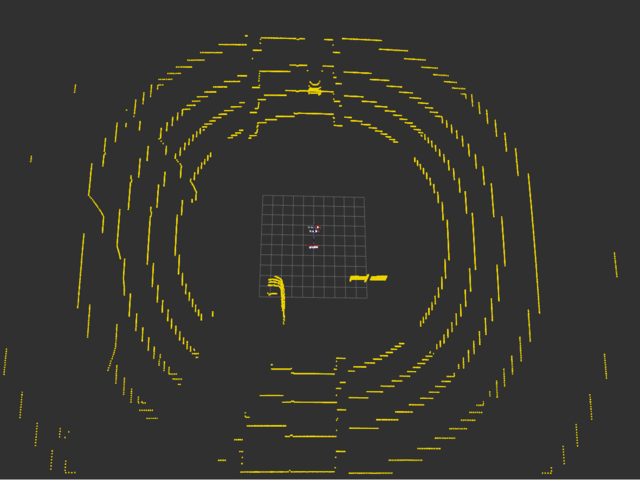
\includegraphics[width=\textwidth]{Figures/Figures_Cap05/pc_objects.png}
         \caption{Antes de aplicar \textit{k-means}.}
         \label{fig:pc_objects}
    \end{subfigure}
    \hfill
    \begin{subfigure}[b]{0.45\textwidth}
         \centering
         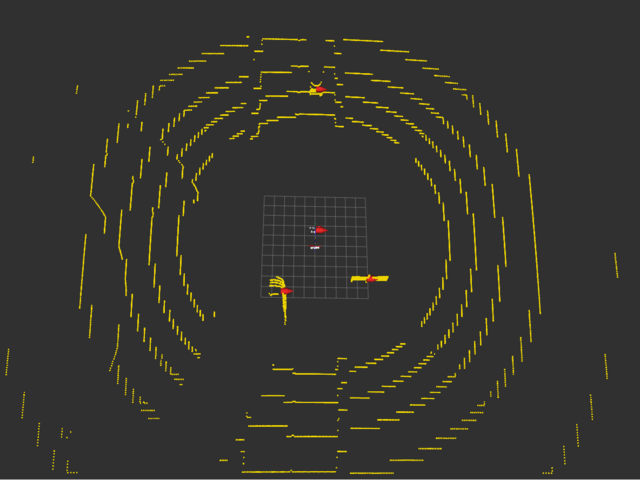
\includegraphics[width=\textwidth]{Figures/Figures_Cap05/pc_centroids.png}
         \caption{Después de aplicar \textit{k-means}.}
         \label{fig:pc_centroids}
     \end{subfigure}
     
    \caption{Nube de puntos antes y después de agrupar mediante \textit{k-means}.}
    \label{fig:pc_clustering}
\end{figure}
%La implementación final de \textit{k-means} en código es en lenguaje C++ debido a los inconvenientes observados con la implementación del mismo algoritmo en Python. En especial se buscó lidiar con el problema de variación de posición para los clusters, para justificar y comprobar este echo se muestra la imagen , donde a y b son el resultado de \textit{k-means} implementado en Python. Es muy notorio que los centroides no son consistentes, si bien detecta los objetos presentes no es posible etiquetar cada centroide con el objeto correspondiente porque cambia constantemente. Por otro lado, con la implementación del mismo algoritmo en C++ se pueden comparar a y b para concluir que los centroides calculados son con
La tarea de detección de objetos concluye al obtener la posición de cada centroide que representa un objeto, este resultado es fundamental para iniciar el proceso de seguimiento de obstáculos.

\section{Empatado} \label{sec:empatado}

Retomando los centroides calculados en \ref{sub:ejemplo_de_implementación_del_algoritmo_K-medias} con el algoritmo de agrupación \textit{k-means} que representan los objetos detectados como la posición media de los puntos de un \textit{cluster} se entiende que conforme el vehículo avanza la nube de puntos cambia en tamaño y forma, como consecuencia el número de centroides varía en cada instante. Este comportamiento presenta la necesidad de saber con certeza que centroide es en cada momento, es decir, se requiere definir si un objeto ha sido previamente detectado con \textit{k-means} y solo ha variado mínimamente su posición. En cambio, si un nuevo objeto es detectado debe ser considerado en la toma de decisiones para evitar colisiones. Dicho de otra forma, el problema por resolver es identificar todos y cada uno de los potenciales obstáculos pues es diferente detectar que identificar objetos. Una vez conocida la posición de los objetos es necesario saber si en cada desplazamiento del vehículo un centroide es el mismo que el anterior o se trata de uno nuevo.

Para empatar dos conjuntos con tamaño $n$ de centroides actual y previo $C_a$ y $C_p$ respectivamente se propone, calcular la distancia euclidiana $d(C_a, C_p)$ entre cada par. 

\begin{equation}
    d(c_{a}, c_{p}) = \sqrt{(c_{a_{x}} - c_{p_{x}})^2 + (c_{a_{y}} - c_{p_{y}})^2 + (c_{a_{z}} - c_{p_{z}})^2}
\end{equation}

Al analizar el resultado de esta operación se obtienen dos posibles escenarios:
\begin{equation}
    d(c_{a}, c_{p}) = \left\lbrace
    \begin{array}{ll}
        \textup{Son el mismo si,} \qquad d(c_{a}, c_{p}) \leq u \\ \\
        \textup{Son diferentes si,} \qquad d(c_{a}, c_{p}) \geq u
    \end{array}
    \right.
\end{equation}
Para el primer caso cuando la distancia $d(c_{a}, c_{p})$ es menor que un umbral $u$ significa que ambos centroides $c_{p}$ y $c_{a}$ representan al mismo objeto, por otro lado cuando la distancia $d(c_{a}, c_{p})$ es mayor que el mismo umbral $u$, implica que $c_{a}$ y $c_{p}$ son dos objetos diferentes. El umbral $u$ es considerado como un valor promedio de las dimensiones de un vehículo pequeño. El algoritmo \ref{alg:matching} describe el empatado de centroides.
\begin{algorithm}
    \begin{algorithmic}[0]
        \REQUIRE Conjunto de centroides previos $C_p$. \\ \parindent=13.5mm Cojunto de centroides actuales $C_a$.
        \ENSURE Conjunto de centroides empatados.
        
        \FORALL{$c_a$} 
            \STATE Obtener el centroide $c$ más cercano a $c_{p}$
            \IF{$d(c, c_a) \geq u$}
                \STATE $c_a$ es un nuevo centroide
                \STATE Agregar $c_a$ al conjunto de centroides empatados.
                %\STATE Crear un nuevo filtro de Kalman con el \textit{id} anterior
            \ELSE
                \STATE $c$ y $c_a$ son el mismo centroide.
            \ENDIF
        \ENDFOR
        \RETURN Conjunto de centroides empatados.
    \end{algorithmic} 
  
    \caption{Algoritmo de Empatado}
    \label{alg:matching}
\end{algorithm}


\section{El filtro de Kalman} \label{sec:el_filtro_de_Kalman}

El filtro de Kalman fue desarrollado por Rudolf E. Kalman en 1960, en principio fue conocido como una solución recursiva al problema de filtrado lineal con datos discretos. En la actualidad es uno de los algoritmos de estimación más importantes y comunes porque produce estimaciones de variables ocultas basadas en mediciones inciertas e inexactas. 
%También, el filtro de Kalman proporciona una predicción del estado futuro del sistema tomando estimaciones pasadas. 

En general, el filtro de Kalman proporciona un método recursivo para estimar el estado futuro de un sistema dinámico en presencia de ruido. El objetivo del filtro es obtener la mejor estimación de un estado \textit{``x''} en el \textit{``k-ésimo''} paso de tiempo dada una estimación previa en combinación con entradas conocidas. Este filtro sirve para estimar estados futuros del sistema cuando se tiene ruido que se adiciona al modelo (ruido de proceso) y a las señales medidas (ruido de medición), además, considera que existe un modelo que relaciona los estados del sistema con las mediciones realizadas (provenientes de los sensores). El proceso de estimación tiene dos dificultades que deben ser superadas. Primero, existe la presencia de vectores de ruido desconocidos e inmedibles. Por lo tanto, una de las tareas es filtrar las perturbaciones no deseadas. La segunda dificultad es que el estado en general no se puede observar directamente desde las salidas previas. Esto significa que la estimación del estado debe reconstruirse en base a la historia temporal de señales y parámetros conocidos \cite{choset2005principles}.

El proceso de estimación mediante el filtro de Kalman es un proceso iterativo y que consta de dos etapas: predicción y actualización: 
\begin{enumerate}
    \item \textbf{Predicción:} En esta etapa el filtro predice el estado, incertidumbre y error siguiente de acuerdo a un modelo del sistema, sin tomar en cuenta el ruido de proceso.
    \item \textbf{Actualización:} Este paso utiliza la información del sensor o sensores utilizados para corregir las estimaciones mediante la diferencia entre valores medidos y valores predichos, posteriormente se calcula una ganancia de Kalman que actualizará los nuevos valores de estado, incertidumbre y error.
    La salida del paso de actualización sirve de retroalimentación al paso de predicción, este proceso continúa hasta que la diferencia entre valor predicho y valor medido tiende a cero.
\end{enumerate}

La figura \ref{fig:kalman_filter_chart} ilustra estos dos pasos.
\begin{figure}[h]
    \centering
    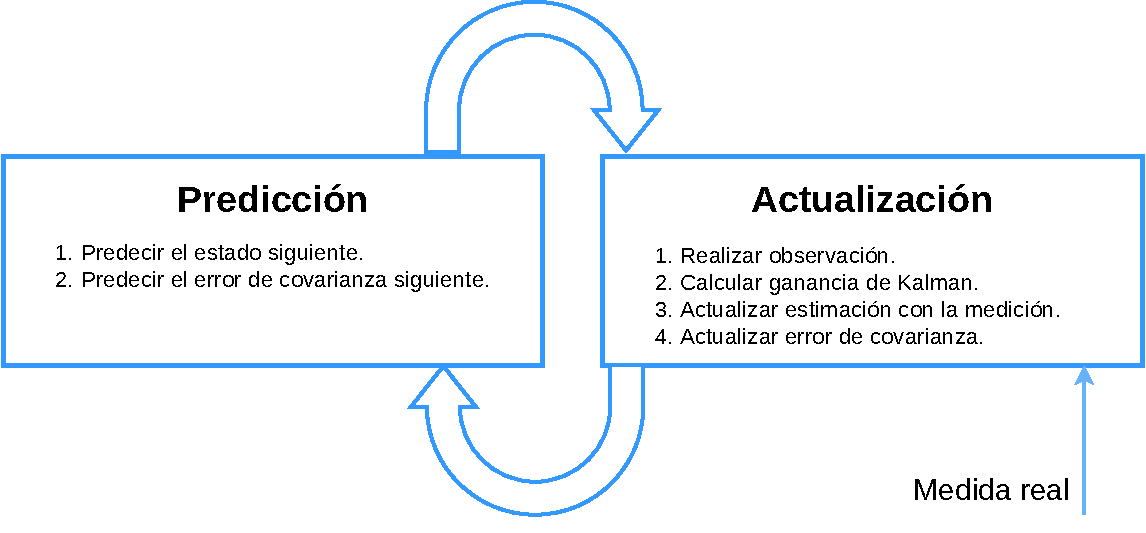
\includegraphics[width=0.75\textwidth]{Figures/Figures_Cap05/kalman_filter_chart.pdf}
    \caption{Etapas del filtro de Kalman.}
    \label{fig:kalman_filter_chart}
\end{figure}

\subsection{El filtro de Kalman extendido} \label{sub:el_filtro_de_Kalman_extendido}

En esencia el filtro de Kalman fue diseñado para estimación de sistemas lineales. Sin embargo, en aplicaciones reales, la mayoría de los sistemas son no lineales, por esta razón, el filtro de Kalman extendido representa una mejora del filtro de Kalman original. El EKF (Extended Kalman Filter) por sus siglas en inglés tiene la facilidad de predecir el estado futuro de un sistema no lineal aplicando métodos de linealización como la matriz jacobiana.

El algoritmo para el filtro de Kalman extendido es descrito con los mismos pasos de predicción y actualización como en el caso de sistemas lineales. Con la diferencia de que en cada estimación de estado, se realiza una linealización del sistema.

\subsection{Estimación de posición y velocidad con el filtro de Kalman extendido} \label{sub:estimación_de_posición_y_velocidad_con_el_filtro_de_kalman_extendido}

El EKF es utilizado en aplicaciones de seguimiento, navegación, control de vehículos y guía. En el caso de un vehículo autónomo se puede usar el filtro para predecir el siguiente movimiento que realizarán los vehículos detectados al frente o los costados de él. El proceso se logra en función de los datos que recibe el vehículo autónomo, específicamente el conjunto de centroides previamente calculados y posteriormente empatados.

Para este trabajo se busca un modelo que permita predecir posición \textit{p} y velocidad \textit{v} de los objetos detectados. En pocas palabras, se busca hacer un seguimiento de objetos (vehículos).
\begin{figure}[h]
    \centering
    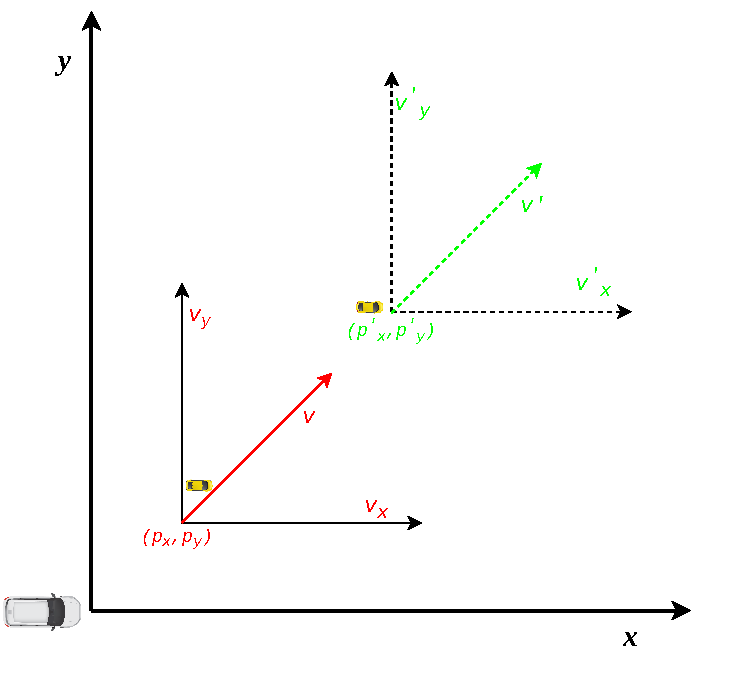
\includegraphics[width=0.75\textwidth]{Figures/Figures_Cap05/ekf_pose_velocity.pdf}
    \caption{Posición y velocidad de un vehículo detectado.}
    \label{fig:ekf_pose_velocity}
\end{figure}

Considerar un entorno 2D como en la imagen \ref{fig:ekf_pose_velocity}, el vehículo autónomo (en color gris) se encuentra en el origen del sistema de referencia $(x, y)$, uno de los posibles vehículos (en color amarillo) detectados previamente, tiene posición $(p_x, p_y)$ y velocidad $(v_x, v_y)$. Dado que se conoce la posición del vehículo detectado se puede obtener la velocidad del mismo como la derivada de la posición $p$ respecto al tiempo $t$. 
\begin{equation*}
    v = \frac{dp}{dt}
\end{equation*}

Mientras que la aceleración es la derivada de la velocidad, en este trabajo se considera velocidad $v$ constante del vehículo detectado en todo momento, por lo tanto, se tiene aceleración $a = 0$

\begin{equation*}
    a = \frac{dv}{dt} = 0
\end{equation*}

De esta manera el sistema por estimar es el siguiente:
\begin{equation*}
    \left\lbrace
    \begin{array}{ll}
        \frac{dp}{dt} = v \\
        \\
        \frac{dv}{dt} = 0
    \end{array}
    \right.
\end{equation*}

y para el caso discreto del modelo anterior se tiene:
\begin{equation*}
    \left\lbrace
    \begin{array}{ll}
        p_{k+1} = p_{k} + \Delta t \hspace{0.1cm} v_{k} + w \\
        \\
        v_{k+1} = v_{k} + w
    \end{array}
    \right.
\end{equation*}

Este sistema permite estimar posición y velocidad de un vehículo detectado. A continuación, se representa este modelo aplicado a la componente $x$ del sistema de referencia de la imagen \ref{fig:ekf_pose_velocity} para fines prácticos. En el caso de la componente $y$ es de la misma forma. Entonces, el sistema de posición y velocidad para la componente $x$ se expresa como:
\begin{equation}
    x=\begin{pmatrix} 
        p_x \\
        v_x
    \end{pmatrix}
    =
    \begin{pmatrix}
        p_{x} + \Delta t \hspace{0.1cm} v_{x} + w \\
        v_{x} + w
    \end{pmatrix}
    \label{eqn:system_pose_vel}
\end{equation}

Y el estado estimado siguiente es:
\begin{equation}
    x'=\begin{pmatrix} 
        p'_x \\
        v'_x
    \end{pmatrix}
    =
    \begin{pmatrix}
        p'_{x} + \Delta t \hspace{0.1cm} v'_{x} + w \\
        v'_{x} + w
    \end{pmatrix}
\end{equation}

donde \textit{x} es el vector de estados, $\Delta t$ es el paso de muestreo, $p_{x}$ y $v_{x}$ son velocidad y posición actual respectivamente y $w$ es ruido de proceso con matriz de covarianza $Q$. El modelo de observación para el filtro es:
\begin{equation}
    z_k = x_k + w
\end{equation}

con $v = 0$, $w$ es ruido de medición con matriz de covarianza $R$. Las mediciones para $z_k$ son las posiciones del conjunto de centroides calculados y empatados. Ahora, la estimación de posición y velocidad consta de los siguientes pasos:

\textbf{Predicción:} Con base en el modelo de posición y velocidad se predice el estado siguiente considerando ruido gaussiano para el modelo de estado y el modelo de medición, como sigue:
\begin{align*} 
    \hat{x}_{k|k-1} &= f(\hat{x}_{k-1|k-1}, u_{k}) \\
    \hat{P}_{k|k-1} &= F_k P_{k-1|k-1} F_{k}^{T} + Q_{k} \\
    \hat{z}_{k|k-1} &= \hat{x}_{k|k-1}
\end{align*}
    
donde $P$ es la matriz de covarianza para el error de estimación, $F_k$ es el Jacobiano (\ref{eqn:f_jacobian}) de la función $f$ (\ref{eqn:system_pose_vel}) y $\hat{z}$ es modelo de observación.
\begin{equation}
    F_k = \begin{pmatrix}
        1 & \Delta t \\
        0 & 1
    \end{pmatrix}
    \label{eqn:f_jacobian}
\end{equation}

Para comenzar la estimación es necesario asignar un valor inicial a la matriz $P$ de ruido de proceso. En este ejemplo $P$ se inicializa con la matriz identidad.

\textbf{Actualización:} La corrección de la estimación se calcula de acuerdo a los errores de observación y estimación. Para el paso de actualización se utilizan las siguientes ecuaciones:
\begin{align*}
    y_k &= z_{k} - h(\hat{x}_{k|k-1}) \\
    S_k &= H_k P_{k|k-1} H_{k}^{T} + R_k \\
    K_k &= P_{k|k-1} H_{k}^T S_{k}^{-1} \\
    \hat{X}_{k|k} &= \hat{x}_{k|k-1} + K_k y_{k} \\
    P_{k|k} &= (I - K_k H_k) P_{k|k-1}
\end{align*}

donde $y_k$ es un residual de medición, $H$ es el Jacobiano (\ref{eqn:h_jacobian}) del modelo de observación respecto a los estados, la matriz $K_k$ es llamada ganancia de Kalman. Las matrices $Q_k$ y $R_k$ para ruido de proceso y ruido de medición respectivamente, son:
\begin{equation*}
    Q_k = \begin{pmatrix}
        0.01 & 0 \\
        0 & 0.01
    \end{pmatrix}
\end{equation*}
y $R_k = 0.1$ es un escalar. El paso de muestreo $\Delta t$ es $0.05 [s]$.
\begin{equation}
    H_k=\begin{pmatrix}
            1 & 0
        \end{pmatrix}
    \label{eqn:h_jacobian}
\end{equation}

Las ecuaciones correspondientes a los pasos de predicción y actualización en forma numérica para la primera iteración son de la forma:

\textbf{Predicción}
\begin{align*}
    \hat{x}&=\begin{pmatrix}1 & \Delta t \\ 0 & 1 \end{pmatrix} \begin{pmatrix} p_x \\ v_x \end{pmatrix} = \begin{pmatrix} p'_{x} \\ v'_{x} \end{pmatrix} \\ \\
    \hat{P}&=\begin{pmatrix} 1 & \Delta t \\ 0 & 1 \end{pmatrix} \begin{pmatrix} 1 & 0 \\ 0 & 1 \end{pmatrix} \begin{pmatrix} 1 & 0 \\ \Delta t & 1 \end{pmatrix} + \begin{pmatrix} 0.01 & 0 \\ 0 & 0.01 \end{pmatrix}
\end{align*}

\textbf{Actualización}
\begin{align*}
    y&=\begin{pmatrix} p_{ox} \\ v_{ox} \end{pmatrix} - \begin{pmatrix} 1 & 0 \end{pmatrix} \begin{pmatrix} p'_{x} \\ v'_{x} \end{pmatrix} \\ \\
    S&=\begin{pmatrix} 1 & 0 \end{pmatrix} \begin{pmatrix} 1 & 0 \\ 0 & 1 \end{pmatrix} \begin{pmatrix} 1 \\ 0 \end{pmatrix} + 0.1 \\ \\
    K&=\begin{pmatrix} 1 & 0 \\ 0 & 1 \end{pmatrix} \begin{pmatrix} 1 \\ 0 \end{pmatrix} \frac{1}{S} \\ \\
    x&=\begin{pmatrix} p'_{x} \\ v'_{x} \end{pmatrix} + K y \\ \\
    P&=\left( \begin{pmatrix} 1 & 0 \\ 0 & 1 \end{pmatrix} - k \begin{pmatrix} 1 & 0    \end{pmatrix} \right) \begin{pmatrix} 1 & 0 \\ 0 & 1 \end{pmatrix}
\end{align*}

Para efectos de implementación en código del Filtro de Kalman Extendido, se optó por crear una clase que contuviera las etapas de predicción y actualización. Después de realizar el proceso de empatado, cada centroide tendrá su propio filtro de Kalman. Mientras $c_a$ y $c_p$ sean el mismo objeto su respectivo filtro de Kalman actualizará posición y velocidad. En el caso de que $c_a$ y $c_p$ sean objetos distintos se creará un nuevo filtro de Kalman para $c_a$.
\newpage

\begin{lstlisting}[language=Python]
# CREATE N OBJECTS
filters = [ [ c, Kalman_Filter() ] for c in centroids ] 

for nc in centroids:
    # COMPUTE DISTANCES
    distances = [ 
        math.sqrt(
            (nc[0] - lc[0])** 2 + 
            (nc[1] - lc[1])** 2 + 
            (nc[2] - lc[2])** 2 
        ) for lc in last_centroids
    ] 
    # GET CLOSER CENTROID (c)
    min_distance = min(distances)
    closer_centroid = last_centroids[
        distances.index(min_distance)
    ]
    closer_idx = distances.index(min_distance)
    if min_distance > threshold: 
        # NC IS A NEW CENTROID, CREATE A NEW OBJECT
        filters[closer_idx] = [ nc, Kalman_Filter() ] 
    else:
        # NC AND C ARE THE SAME, UPDATE MEASURE
        filters[closer_idx][0] = nc 

# APPLY EKF TO FILTERS MATCHED
for c,kalman_filter in filters:
    kalman_filter.ekf(c)
\end{lstlisting}
\hfill

La porción de código anterior representa las tareas de empatado de centroides y estimación de posición y velocidad con el EKF. Al inicio (línea 2) se crean $n$ filtros de Kalman para los objetos detectados. Posteriormente, a partir de la línea 4 y hasta la línea 24 se implementa el algoritmo \ref{alg:matching} para el empatado de centroides actuales y previos. Finalmente, las líneas 27 y 28 efectúan el proceso de filtrado de posición y velocidad con Kalman. Donde la línea 18 hace uso de la clase 'Kalman\_Filter' que calcula cada una de las ecuaciones para predicción y actualización.

Anteriormente, en la sección \ref{sec:simuladores} y en específico con la figura \ref{fig:pc_clustering} se mostró el resultado de la detección de objetos mediante el algoritmo de clusterización \textit{k-means}. La imagen \ref{fig:object_detect_tracking} es una visualización con RViz que muestra la conclusión de empatar centroides y realizar una estimación de posición y velocidad con el filtro de Kalman extendido, a cada objeto se le asigna una etiqueta con sus correspondientes valores de posición y velocidad $[x, z]$ filtrados. En \ref{fig:object_tracking_static} se ilustra el seguimiento de objetos estáticos, se estima la posición $p[x, z]$ de un objeto mientras que la velocidad $v[x, z] = [0, 0]$. El caso de seguimiento de objetos en movimiento se muestra en \ref{fig:object_tracking_dynamic} donde; la velocidad $v[x, z] \neq [0, 0]$. Es importante mencionar que las velocidades del vehículo solo aparecen en la componente $z$ porque los vehículos en seguimiento se desplazan solo en dirección vertical.

\begin{figure}[h]
    \centering
    \begin{subfigure}[b]{0.4\textwidth}
         \centering
         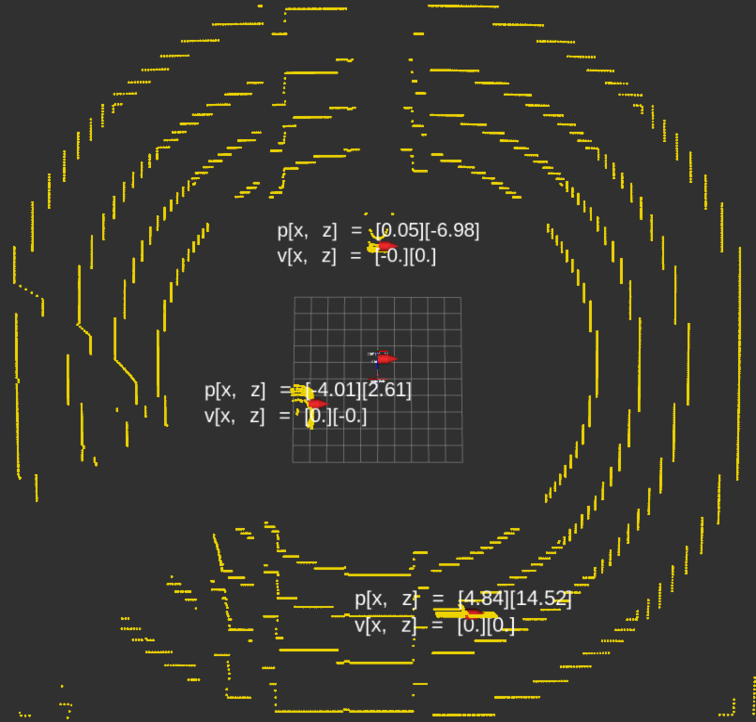
\includegraphics[width=\textwidth]{Figures/Figures_Cap05/object_tracking_static.png}
         \caption{Seguimiento de objetos estáticos.}
         \label{fig:object_tracking_static}
    \end{subfigure}
    \hfill
    \begin{subfigure}[b]{0.4\textwidth}
         \centering
         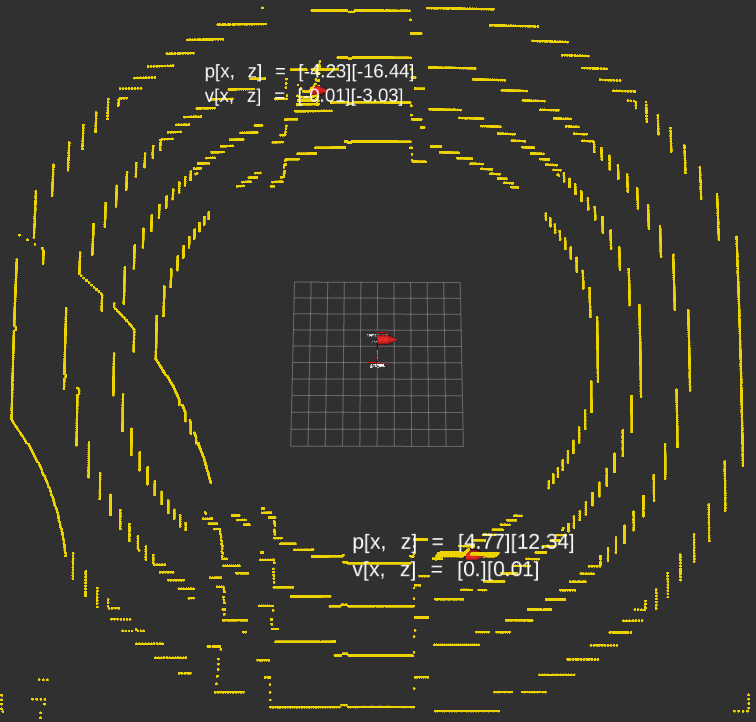
\includegraphics[width=\textwidth]{Figures/Figures_Cap05/object_tracking_dynamic.png}
         \caption{Seguimiento de objetos dinámicos.}
         \label{fig:object_tracking_dynamic}
     \end{subfigure}
     
    \caption{Seguimiento de objetos estáticos y dinámicos.}
    \label{fig:object_detect_tracking}
\end{figure}
\newpage

% CONCLUSIONES DEL CAPÍTULO
Al finalizar este capítulo el vehículo de pruebas cuenta con un sistema de navegación más completo, al incluir detección de objetos con ayuda de \textit{k-means} y seguimiento de objetos con el filtro de Kalman extendido se puede añadir más complejidad al escenario de pruebas descrito en \ref{sec:el_ambiente_de_simulación} y utilizado en el capítulo anterior. En primer lugar, con la aparición de nuevos vehículos en distintas posiciones y en algunos casos con velocidades controladas. Anteriormente, el vehículo autónomo solo podía navegar en un ambiente sin obstáculos utilizando las líneas del carril como guía. En este punto el vehículo aún no es capaz de navegar de manera segura en un ambiente que presente obstáculos, pero con la inclusión de detección y seguimiento de vehículos el vehículo autónomo cuenta con una mejor percepción del ambiente.

En el capítulo siguiente serán esenciales las implementaciones recién añadidas más las del capítulo \ref{cap:seguimiento_de_carriles}, esto con el objetivo de diseñar e implementar diferentes comportamientos y estrategias que le permitan al vehículo autónomo navegar por el circuito que ahora cuenta con obstáculos. Además, se buscarán definir reglas para la toma decisiones en situaciones cercanas a la realidad.

